	\section*{Exercice 4 (5 points)}
	
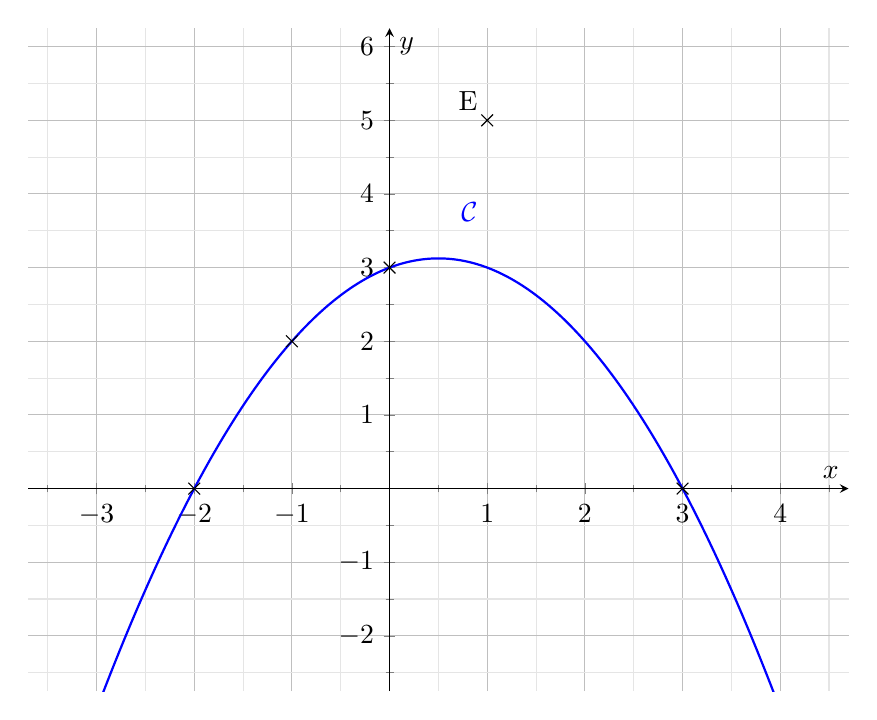
\begin{tikzpicture}
	\begin{axis}[
		axis lines = center,
		grid = both,
		xmin = -3, xmax = 4,
		ymin = -2, ymax = 5.5,
		xlabel = {$x$},
		ylabel = {$y$},
		domain = -3:4,
		samples = 200,
		enlargelimits,
		xtick distance = 1,
		ytick distance = 1,
		grid style = {line width = 0.4pt, draw = gray!20},
		major grid style = {line width = 0.4pt, draw = gray!50},
		minor tick num = 1,
		width = 12cm,
		height = 10cm,
		]
		
		\addplot[
		thick,
		blue,
		]
		{0.5*(6 + x - x^2)};
		
		\addplot[
		only marks,
		mark = x,
		mark size = 3,
		]
		coordinates {
			(3,0)
			(-2,0)
			(-1,2)
			(0,3)
			(1,5)
		};
		
		\node[anchor=south east] at (axis cs:1,5) {E};
		\node[anchor=south east, blue] at (axis cs:1,3.5) {$\mathcal{C}$};
		
	\end{axis}
\end{tikzpicture}
	
	\subsection*{1. Par lecture graphique, résoudre l’équation $f(x) = 0$ d’inconnue $x$.}
	
On voit que la courbe coupe l’axe des abscisses aux points d’abscisses $-2$ et $3$. \\
	Donc $S = \{-2; 3\}$.
	
	\subsection*{2. On donne $f'(x) = -x + 0,5$ pour tout réel $x$. Déterminer qu’une équation de la tangente $T$ à la courbe $C$ au point d’abscisse $-1$ est $y = 1,5x + 3,5$.}
	
On lit $f(-1) = 2$ et d’après l’indication $f'(-1) = 1 + 0,5 = 1,5$.\\
Une équation de la tangente à la courbe au point d’abscisse $-1$ est donc :
	\[
	y - f(0) = f'(0)(x - 1), \text{ soit } y - 2 = 1,5(x + 1) \text{ ou } y = 2 + 1,5x + 1,5 \text{ et finalement } y = 1,5x + 3,5
	\]
	
	\subsection*{3. On considère le point $E$ de coordonnées $(1; 5)$. Dans cette question, on cherche à déterminer les points de la courbe $C$ en lesquels la tangente passe par le point $E$.}
	
	\subsubsection*{a. Montrer que le point $E$ appartient à la tangente $T$.}
	
$E(1; 5) \in T \Leftrightarrow 5 = 1,5 \times 1 + 3,5$ soit si $5 = 1,5 + 3,5$ ce qui est vrai.
	
	\subsubsection*{b. Déterminer l’autre point de la courbe en lequel la tangente passe par le point $E$.}
	
La première question incite à considérer le point de coordonnées $(3; 0)$ de la courbe.\\
Une équation de la tangente $T_3$ à la courbe en ce point avec \\
$f(3) = 0$ et $f'(3) = -3 + 0,5 = -2,5$ est :
\[	y - 0 = -2,5(x - 3), \text{ soit } y = -2,5(x - 3)
	\]
	
Or pour $x = 1$, $y = -2,5(1 - 3) = -2,5 \times (-2) = 5$, donc cette tangente contient le point $E$.\\
 Les tangentes à la courbe contenant $E$ sont donc les tangentes en $(-1; 2)$ et $(3; 0)$.
	
